\begin{figure*}[htbp]
   \centering
   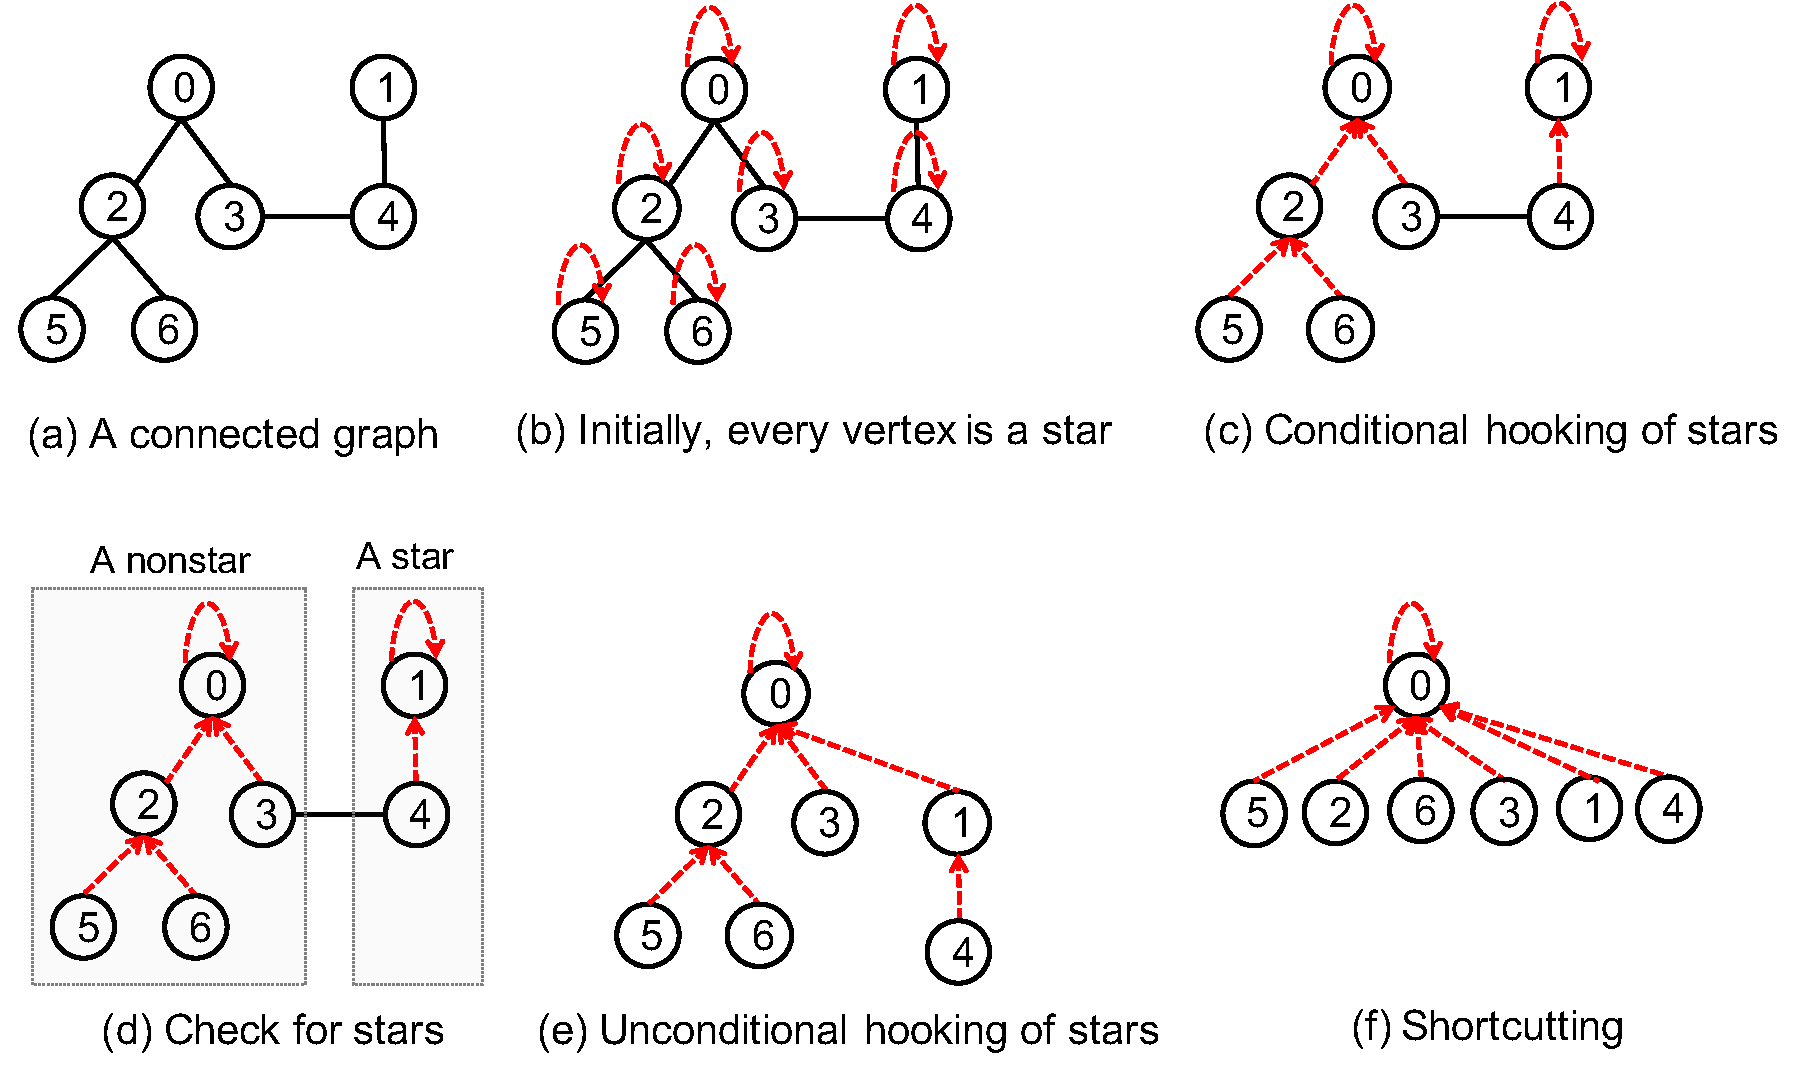
\includegraphics[scale=.45]{figures/example} % requires the graphicx package
   \caption{example caption}
   \label{fig:example}
\end{figure*}



\begin{figure*}[htbp]
   \centering
   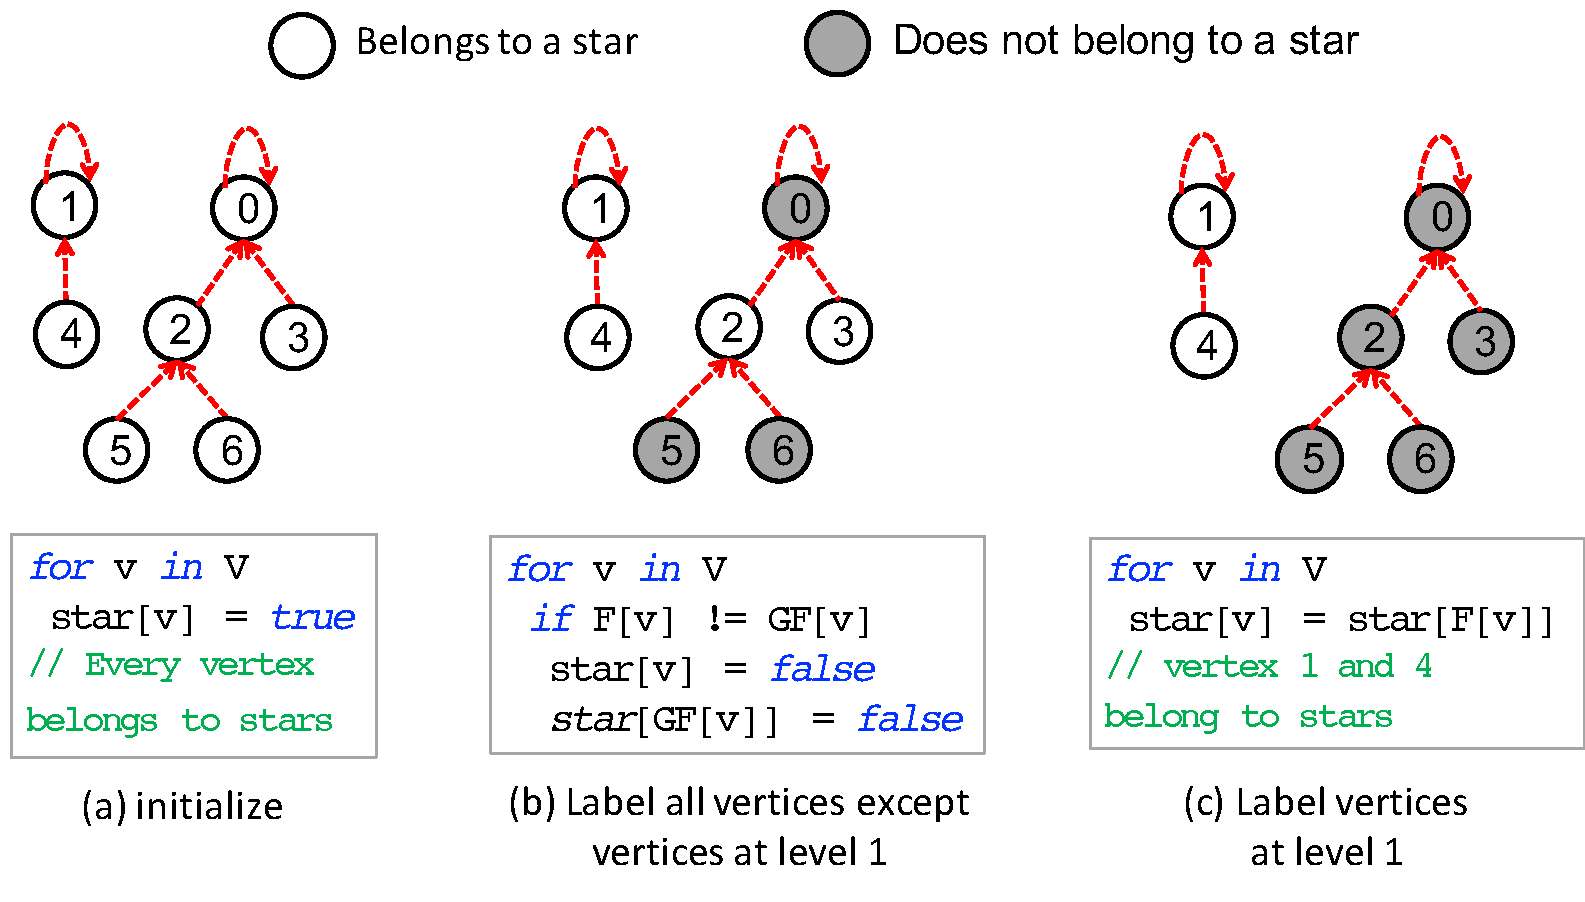
\includegraphics[scale=.45]{figures/starcheck} % requires the graphicx package
   \caption{example caption}
   \label{fig:starcheck}
\end{figure*}


\begin{algorithm}[htbp]
\begin{algorithmic}[1]
\begin{small}
\Procedure{Awerbuch-Shiloach}{$G(V,E), f$}
	\LineComment{\textcolor{blue}{Initialization }}
	\For {every vertex $v$ in $V$}
		\State $f[v] \gets u$
	\EndFor
	
	\Repeat
	\LineComment{\textcolor{blue}{Step1: Conditional star hooking }}
	\For {every edge \{$u,v$\} in $E$} {\bf in parallel }
		\If {$u$ belongs to a star and $f[u] > f[v]$}
		\State $f[f[u]] \gets f[v]$
		\EndIf
	\EndFor
	\LineComment{\textcolor{blue}{Step2: Unconditional star hooking }}
	\For {every edge \{$u,v$\} in $E$} {\bf in parallel }
		\If {$u$ belongs to a star and $f[u] \neq f[v]$}
		\State $f[f[u]] \gets f[v]$
		\EndIf

	\EndFor
	\LineComment{\textcolor{blue}{ Step3: Shortcutting}}
	\For {every vertex $v$ in $V$} {\bf in parallel }
		\State \id{gf}$[v] \gets f[f[v]]$
	\EndFor
	\For {every vertex $v$ in $V$} {\bf in parallel }
		\If {$v$ does not belongs to a star}
		\State $f[v] \gets  \id{gf}[v]]$
		\EndIf
	\EndFor
	\Until{$f$ reamins unchanged}
\EndProcedure
\end{small}
\end{algorithmic}
\caption{The skeleton of the Awerbuch-Shiloach algorithm.}
\label{algo:Awerbuch-Shiloach}
\end{algorithm}


\begin{algorithm}[htbp]
\begin{algorithmic}[1]
\begin{small}
\Procedure{Starcheck}{$G(V,E), f$}
	\LineComment{\textcolor{blue}{Initialization }}
	\For {every vertex $v$ in $V$} {\bf in parallel }
		\State $star[v] \gets true$
		\State \id{gf}$[v] \gets f[f[v]]$
	\EndFor
	
	\LineComment{\textcolor{blue}{Exclude vertices at depth greater than 1 and roots of nonstars }}
	\For {every vertex $v$ in $V$} {\bf in parallel }
		\If {$f[v] \neq \id{gf}[v]$}
			\State $star[v] \gets false$
			\State $star[\id{gf}[v]] \gets false$
		\EndIf
	\EndFor
	
	\LineComment{\textcolor{blue}{Exclude vertices at depth =1 in nonstar trees}}
	\For {every vertex $v$ in $V$} {\bf in parallel }
		\State $star[v] \gets star[f[v]]$
	\EndFor
	
\EndProcedure
\end{small}
\end{algorithmic}
\caption{Finding vertices belonging to stars.}
\label{algo:Starcheck}
\end{algorithm}


\section{The Awerbuch-Shiloach algorithm}
The Awerbuch-Shiloach algorithm maintains a forest data structure where each tree represents a connected component at the current stage of the algorithm.
A tree is called a \emph{star} if every vertex is a child of the root (i.e., the height of three is at most one).
The Awerbuch-Shiloach algorithm begins with singleton trees (stars) corresponding to each vertex in the graph.
In every iteration, we merge stars with other trees (both star and nonstars) until no such merging is possible. 
This merging is called ``hooking" in the Awerbuch-Shiloach algorithm and is performed in two steps: (a) conditional hooking and (b) unconditional hooking. These steps are described below.
Between two subsequent iterations, the algorithm reduces the hight of trees by pointer jumping, a process known as shortcutting. 
Note that the Awerbuch-Shiloach algorithm is a simplification of the Shiloach-Vishkin algorithm~\cite{shiloach1980log}. While Shiloach-Vishkin allows hooking a tree to another tree, Awerbuch-Shiloach only allows hooking a star onto another tree. Hooking stars instead of trees simplifies the hooking process and eliminate the need of some auxiliary data structures needed by the Shiloach-Vishkin algorithm.

In the Awerbuch-Shiloach algorithm, vertex $u$ maintains a parent $f[u]$ which is another vertex or itself. 
This parent-child relationship forms a directed forest where the root $u$ of a tree satisfies $f[u]=u$.
Algorithm \ref{algo:Awerbuch-Shiloach} describes the overview of the Awerbuch-Shiloach algorithm.
Initially every vertex forms a separate star. 
In each iteration, the algorithm performs three steps conditional (a) conditional hooking, (b) unconditional hooking and (c) shortcutting.
Each of these three steps can be done in parallel as shown in Algorithm \ref{algo:Awerbuch-Shiloach}.
Figure~\ref{fig:example} shows the execution of different steps of the Awerbuch-Shiloach algorithm.

Algorithm~\ref{algo:Starcheck} is used to identify vertices belonging to stars.
Figure~\ref{fig:starcheck} shows a running example of finding vertices in stars in the trees from Figure~\ref{fig:example}(d).

The Awerbuch-Shiloach algorithm terminates when every tree becomes a star and the parent array is not updated in the latest iteration. 
Awerbuch and Shiloach showed that the algorithm terminates in $O(\log n)$ iterations. Hence, using $m+n$ processors, the algorithm has $O(\log n)$ complexity in a PRAM model. 




\section{The Awerbuch-Shiloach algorithm using GraphBLAS primitives}
\label{sec:LACC}
At first, we design the Awerbuch-Shiloach algorithm in the language of sparse linear algebra.
For this purpose, we relied upon several GraphBLAS primitives as defined in its C API~\cite{bulucc2017design}.
The implementation details of these primitives (using the Combinatorial BLAS library) will be discussed in the next section.

We use three GraphBLAS operations to design the Awerbuch-Shiloach algorithm: (a) GrB\_mxv to perform sparse matrix-vector multiplication, (b) GrB\_extract for extracting some elements of a vector and (c) GrB\_assign for assigning elements of a vector to a destination vector. 
The conditional and unconditional hooking operations in the Awerbuch-Shiloach algorithm traverses the neighbors of a subset of vertices  in the graph. This operation can be captured by sparse matrix-vector (SpMV) product on an appropriate semiring.  
We refer to a semiring by listing its scaling operations, such as the (multiply, add) semiring. 
In LACC, we use Select2nd as semiring multiply, which returns the second value it is passed. 
We use min as semiring add, which returns the minimum of the two operand it is passed.
Hence, we use (Select2nd, min) semiring throughout our SpMV algorithms. 
Algorithm~\ref{algo:Sel2ndMin} describes how this semiring can be created using GraphBLAS C API.
The BFS semiring is defined
over two sets: the matrix elements are from the set of binary
numbers whereas the vector elements are from the set of
integers.

\begin{algorithm}[htbp]
\begin{algorithmic}[1]
\begin{small}
\Procedure{Semiring}{$\lvert V \rvert$}
	\State GrB\_Monoid Min
	\State GrB\_Monoid\_new(\&Min, GrB\_MIN, $\lvert V \rvert$)
	\State GrB\_Semiring Sel2ndMin
	\State GrB\_Semiring\_new(\&Sel2ndMin, Min, GrB\_SECOND)
	\State \Return Sel2ndMin
\EndProcedure
\end{small}
\end{algorithmic}
\caption{Create a semiring with (multiply, add) operations replaced by (Select2nd, min)}
\label{algo:Sel2ndMin}
\end{algorithm}



\subsection{Conditional hooking}
Algorithm~\ref{algo:condHook} describes how we designed the conditional hooking using three GraphBLAS operations.
GrB\_mxv in  Algorithm~\ref{algo:condHook} multiply the adjacency matrix $\mA$ of the graph by the parent vector $f$ on a (Select2nd, min) semiring. Since we only care about output vertices belonging to stars, we masked the output in GrB\_mxv by the Boolean vector \id{star}.
The output of GrB\_mxv is stored in $f_n$.  $f_n[v]$ stores the minimum parent of an adjacent vertex of $v$ where \id{star[v]} is true.  
Next, the GrB\_extract function extracts the parents of vertices in a star. Here we again use the \id{star} vector as an output mask.
Finally, the GrB\_assign function updates the parents of the roots of stars when possible.

\begin{algorithm}[htbp]
\begin{algorithmic}[1]
\begin{small}
\Procedure{CondHook}{$\mA$, $f$, \id{star}}
	\State Sel2ndMin $\gets$ \Call{Semiring}{$\lvert V \rvert$}
	\LineComment{\textcolor{blue}{Step1: For every vertex in a star, find a neighbor with the minimum parent id. SpMV($\mA$,  $f$) with the Sel2ndMin semiring and the output masked by \id{star} does the job. $f_n$ is the output vector. }}
	\State GrB\_mxv ($f_n$, \id{star},  GrB\_NULL,  Sel2ndMin,  $\mA$,  $f$, GrB\_NULL) \li
	\LineComment{\textcolor{blue}{Step2: Extract parents of vertices in stars ($f_{star} = f[star]$). We use GrB\_extract to extract from the parent array $f$ using \id{star} as a mask.}}
	\State GrB\_extract ($f_{star}$, \id{star},GrB\_NULL,  $f$,  GrB\_ALL, 0, GrB\_NULL) 
	\LineComment{\textcolor{blue}{Step3: Hook root of a star  to a neighboring tree ($f[f_{star}] = f_n$}).}
	\State GrB\_assign ($f$, GrB\_NULL,  GrB\_NULL,  $f_n$,  $f_{star}$,  size($f_{star}$), GrB\_NULL) 

 	%$F_n \gets$ \Call{SpMV}{$\mA, F $, SR=(select2nd, min)}  \tcp*{minimum father among all neighbors} 
	%F[V_star] = F_n[V_star]
	%GrB_extract(, star, GrB_NULL, GrB_ALL)
 \EndProcedure
\end{small}
\end{algorithmic}
\caption{Conditional hooking of stars onto other trees (both stars and non stars).  {\bf Inputs:} a sparse adjacency matrix $\mA$, a dense vector $f$ storing the parents of all vertices, a dense Boolean vector $stars$ storing whether the $i$th vertex belongs to a star.
{\bf Output:} Updated parent array $f$.}
\label{algo:condHook}
\end{algorithm}

\subsection{Unconditional hooking}
Algorithm~\ref{algo:uncondHook} describes how we designed the unconditional hooking using three GraphBLAS operations.
As shown in Algorithm~\ref{algo:Awerbuch-Shiloach},  unconditional hooking is very similar to conditional hooking  with the only different is that unconditional hooking allows a star to hook with any other tree without any restriction on the order of vertices.
However, unlike conditional hooking where a star can hook to another star or nonstar, conditional hooking enables hooking a star onto a nonstar only. 
This allows us to use a sparse vector $f_{nonstar}$ as an input to GrB\_mxv, where $f_{nonstar}$ is the subset of vertices belonging to nonstar trees. 
Hence, GrB\_mxv in  Algorithm~\ref{algo:uncondHook} multiply the adjacency matrix $\mA$ of the graph by the sparse vector $f_{nonstar}$ on a (Select2nd, min) semiring. 
In fact, (Select2nd, min) semiring is not strictly required here since the order of parents does not matter in unconditional hooking.
As before, we masked the output in GrB\_mxv by the Boolean vector \id{star}.
The output of GrB\_mxv is stored in $f_n$.  $f_n[v]$ stores the minimum parent of an adjacent vertex $w$ of $v$ where \id{star[v]} is true and \id{star[w]} is false.  
Next, the GrB\_extract function extracts the parents of vertices in a star. Here we again use the \id{star} vector as an output mask.
Finally, the GrB\_assign function updates the parents of the roots of stars when possible.


\begin{algorithm}[htbp]
\begin{algorithmic}[1]
\begin{small}
\Procedure{UncondHook}{$\mA$, $f$, \id{star}}
	\State Sel2ndMin $\gets$ \Call{Semiring}{$\lvert V \rvert$}
	\LineComment{\textcolor{blue}{Step1: Extract parents of vertices not in stars. We use GrB\_extract to extract from the parent array $f$ using the structural complement of \id{star} as a mask.}}
	\State GrB\_extract($f_{nonstar}$, \id{star},GrB\_NULL,  $f$,  GrB\_ALL, 0, GrB\_SCMP) 
	
	\LineComment{\textcolor{blue}{Step2: For every vertex in a star, find a neighbor in a nonstar. SpMV($\mA$,  $f_{nonstar}$) with the Sel2ndMin semiring and the output masked by \id{star} does the job. $f_n$ is the output vector. Min is used just to break ties. Selecting any of the two operands is sufficient here. }}
	\State GrB\_mxv ($f_n$, \id{star},  GrB\_NULL,  Sel2ndMin,  $\mA$,  $f_{nonstar}$, GrB\_NULL) 
	\LineComment{\textcolor{blue}{Step2: Extract parents of vertices in stars ($f_{star} = f[star]$). We use GrB\_extract to extract from the parent array $f$ using \id{star} as a mask.}}
	\State GrB\_extract ($f_{star}$, \id{star},GrB\_NULL,  $f$,  GrB\_ALL, 0, GrB\_NULL) 
	\LineComment{\textcolor{blue}{Step3: Hook root of a star  to a neighboring tree ($f[f_{star}] = f_n$}).}
	\State GrB\_assign ($f$, GrB\_NULL,  GrB\_NULL,  $f_n$,  $f_{star}$,  size($f_{star}$), GrB\_NULL) 

 	%$F_n \gets$ \Call{SpMV}{$\mA, F $, SR=(select2nd, min)}  \tcp*{minimum father among all neighbors} 
	%F[V_star] = F_n[V_star]
	%GrB_extract(, star, GrB_NULL, GrB_ALL)
 \EndProcedure
\end{small}
\end{algorithmic}
\caption{Unconditional hooking of stars onto other trees (only non stars).  {\bf Inputs:} a sparse adjacency matrix $\mA$, a dense vector $f$ storing the parents of all vertices, a dense Boolean vector $stars$ storing whether the $i$th vertex belongs to a star.
{\bf Output:} Updated parent array $f$.}
\label{algo:uncondHook}
\end{algorithm}


\begin{algorithm}[htbp]
\begin{algorithmic}[1]
\begin{small}
\Procedure{Shortcut}{$f$}
	\LineComment{\textcolor{blue}{Step1: find grandfathers ($\id{gf} \gets f[f] $) }}
	\State GrB\_extract (\id{gf}, GrB\_NULL, GrB\_NULL,  $f$,  $f$, 0, GrB\_NULL) 
	\LineComment{\textcolor{blue}{Step2:  $f \gets \id{gf}$}).}
	\State GrB\_assign ($f$, GrB\_NULL,  GrB\_NULL,  GrB\_ALL,  \id{gf},  size($f$), GrB\_NULL) 
 \EndProcedure
\end{small}
\end{algorithmic}
\caption{Shortcutting using GrB\_extract and GrB\_assign.  {\bf Inputs:} a dense vector $f$ storing the parents of all vertices.
{\bf Output:} Updated parent array $f$.}
\label{algo:shortcut}
\end{algorithm}


\subsection{Shortcutting}
Algorithm~\ref{algo:shortcut} describes how we designed the shortcutting using two GraphBLAS operations.
At first, we use  GrB\_extract to obtain the grand parent \id{gf} of every vertex. Next, we assign \id{gf} to the parent array by using the GrB\_assign operation.


\section{Implementing the Awerbuch-Shiloach algorithm in CombBLAS}
We use the CombBLAS framework~\cite{bulucc2011combinatorial} to implement the GraphBLAS primitives needed to implement the Awerbuch-Shiloach algorithm.
Since CombBLAS does not directly support the masking operations, we filtered out the output after performing an operation (if masking is needed). 

CombBLAS distributes its sparse matrices on a 2D $p_r \times p_c$ processor grid.
Processor $P(i,j)$ stores the submatrix $\mA_{ij}$ of dimensions $(m/p_r)\times (n/p_c)$ in its local memory. 
The CombBLAS uses the doubly compressed sparse columns (DCSC) format to store its local submatrices for scalability, 
and uses a vector of \{index, value\} pairs for storing sparse vectors. 
To balance load across processors, we randomly permute the input matrix $\mA$ before running the matching algorithms.

Vectors are also distributed on the same 2D processor grid. 
For a distributed vector $v$, the syntax $v_{ij}$ denotes the local $n/p$ length piece of the vector owned by the $P(i, j)$th processor. 
The syntax $v_i$ denotes the hypothetical $n/p_r$ or $n/p_c$ length piece of the vector collectively owned by all the processors along the $i$th processor row $P(i, :)$ or column $P(:, i)$.


\subsection{Analysis of the distributed algorithm}
We measure communication by the number of {\em words} moved ($W$) and
the number of {\em messages} sent ($S$). The cost of communicating a length $m$ message is $\alpha + \beta m$ where $\alpha$ is the
latency and $\beta$ is the inverse bandwidth, both defined relative to the cost of a single arithmetic operation. Hence, an algorithm that
performs $F$ arithmetic operations, sends $S$ messages, and moves $W$ words takes $T= F + \alpha S + \beta W$ time. 

We previously analyzed~\cite{azad2016distributed} the complexity of SpMV because it is also a building block of parallel maximal matching algorithms.
For ease of analysis, we assume that nonzeros are i.i.d. distributed in matrices and vectors. %,  $x$ is $\id{f}$ percent full, and $\mA$ has on average $d$ nonzeros per column. 
We also assume a square processor grid $p_c{=}p_r{=}\sqrt{p}$. Number of iterations is denoted by $\left\vert{\mathrm{iters}} \right\vert$.

%We leverage the 2D SpMV algorithms implemented in CombBLAS.
%The complexity of the parallel SpMSpV algorithm has been analyzed in this context recently~\cite{matchingipdps16}, hence we just state
%the result here: 
% $$ T_{ \Call{SpMV}{}}  = O \Bigl( \frac{m}{p} +  \beta  \bigl ( \frac{m}{p} + \frac{n}{\sqrt{p}} \bigr ) +  \left\vert{\mathrm{iters}} \right\vert \alpha \sqrt{p} \Bigr) .$$
 






